
\section{Calculations \& Graphs}

\vspace{-0.5cm}
\singlespacing

%------- Force --------%

\subsection{Center of Mass} 

{\centering
\begin{equation}
	x_\text{com} = \frac{m_1x_1 + m_2x_2 + ...}{M_T} 
	\label{eq:COM}
\end{equation}
\begin{align*}
	x_\text{com} &: \text{center of mass} \\
	m_1 &: \text{mass of object 1} \\
	m_2 &: \text{mass of object 2} \\
	x_1 &: \text{position of object 1} \\
	x_2 &: \text{position of object 2} \\
	M_T &: \text{total mass of system}
\end{align*}}

\subsubsection{Sample Calculation \\ {\normalfont \small\textit{using values from Scenario 1}}}

{\centering
\begin{align*}
	x_\text{com} &= \frac{m_1x_1 + m_2x_2 + ...}{M_T} \\ \\
							 &= \frac{(0.06\text{ kg})(0.8\text{ m}) + (0.1\text{ kg})(0.333\text{ m})}{(0.16\text{ kg})} \\ \\ 
	x_\text{com} &= \boxed{0.509 \text{ m}} 
\end{align*}}

%------- ACCELERATION BETWEEN TWO POINTS WITH INITIAL VELOCITY CLOSE TO ZERO--------%



%------- ACCELERATION BETWEEN TWO POINTS --------%

%------- AVERAGE VALUE --------%
%------- AVERAGE VALUE --------%

%------- STANDARD DEVIATION --------%
%\subsection{Standard Deviation Formula}
%
%\begin{align*}
%		\sigma &= \sqrt{\frac{\Sigma(x_i -\overline{a})^2}{N}} \\
%		 &= \sqrt{\frac{SS}{N}} \\ \\
%		\textbf{N} &:\, \text{Total number of values} \\
%		\overline{\textbf{a}} &:\, \text{Average value} \\
%		\textbf{x\textsubscript{i}} &:\, \text{Each value from the data set} \\
%		\textbf{SS} &:\, \text{Sum of squares} 
%\end{align*}
%
%\subsubsection{Sample Calculation \\ {\normalfont \small\textit{std of photogate times with hanging mass at 10 grams }}}
%
%\begin{align*}
%	\sigma &= \sqrt{\frac{(1.461-\overline{a})^2 + ... + (1.454-\overline{a})^2}{3}} \\
%				 &= \sqrt{\frac{2.886\,\text{x}\,10^{-5}}{3}} \\
%		 &= \boxed{0.0003\, \text{s}}
%\end{align*}
%------- STANDARD DEVIATION --------%

%------- RELATIVE ERROR --------%
\subsection{Percent Error}
\vspace{0.5cm}
\begin{equation}
	\text{PD}	= \left| \frac{\text{measured - actual}}{\text{actual}} \right|\: \text{x}\: 100\%
	\label{eq:perror}
\end{equation}

\subsubsection{Sample Calculation \\ {\normalfont \small\textit{percent error between measured and calculated position for 100 g in Scenario 1}}}

\begin{align*}
	\text{PD}	&= \left| \frac{\text{measured - actual}}{\text{actual}} \right|\: \text{x}\: 100\% \\ \\
	\text{PD}	&= \left| \frac{\text{0.333\text{ m} - 0.334\text{ m}}}{\text{0.334\text{ m}}} \right|\: \text{x}\: 100\% \\ \\
	\text{PD} &= \boxed{0.29\%} 
\end{align*}

%------- RELATIVE ERROR --------%

%----TABLES-----%
\subsection{Graphs \& Tables}

\begin{figure}[H]
	\captionsetup{font=large}
	\caption{Scenario 1}\label{fig:Scenario1}
	\begin{center}
		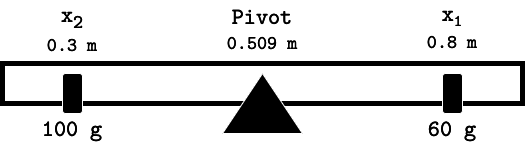
\includegraphics[width=0.75\textwidth]{Scenario1.png}
	\end{center}
\end{figure}

\vspace{-0.5cm}

\begin{table}[H]
\centering
\captionsetup{font=large}
\caption{Scenario 1 - Values}
\label{tab:s1tab}
\resizebox{11cm}{!}{%
\begin{tabular}{@{}cccc@{}}
\toprule
\multicolumn{2}{c}{\textbf{x\textsubscript{com} (m)}}      & 0.509  &                      \\ \midrule
\textbf{x\textsubscript{1} (m)}          & \multicolumn{1}{c|}{0.8}    & \textbf{m\textsubscript{1} (kg)} & 0.06 \\
\textbf{x\textsubscript{2} Actual (m)}   & \multicolumn{1}{c|}{0.333}  & \textbf{m\textsubscript{2} (kg)} & 0.1  \\
\textbf{x\textsubscript{2} Expected (m)} & \multicolumn{1}{c|}{0.3344} & \textbf{M\textsubscript{T} (kg)} & 0.16 \\ \midrule
\multicolumn{2}{c}{\textbf{x\textsubscript{2} Error (\%)}} & 0.4186 & \multicolumn{1}{l}{} \\ \bottomrule
\end{tabular}%
}
\end{table}


\begin{figure}[H]
	\captionsetup{font=large}
	\caption{Scenario 2}\label{fig:Scenario2}
	\begin{center}
		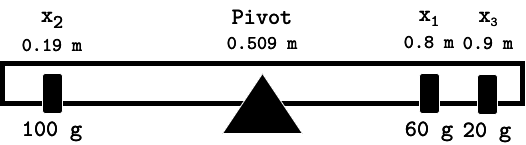
\includegraphics[width=0.75\textwidth]{Scenario2.png}
	\end{center}
\end{figure}

\vspace{-0.5cm}

\begin{table}[H]
\centering
\captionsetup{font=large}
\caption{Scenario 2 - Values}
\label{tab:s2tab}
\resizebox{11cm}{!}{%
\begin{tabular}{@{}cccc@{}}
\toprule
\multicolumn{2}{c}{\textbf{x\textsubscript{com} (m)}}      & 0.509                            &      \\ \midrule
\textbf{x\textsubscript{1} (m)} & \multicolumn{1}{c|}{0.83} & \textbf{m\textsubscript{1} (kg)} & 0.06 \\
\textbf{x\textsubscript{2} Actual (m)}   & \multicolumn{1}{c|}{0.19}   & \textbf{m\textsubscript{2} (kg)} & 0.1  \\
\textbf{x\textsubscript{2} Expected (m)} & \multicolumn{1}{c|}{0.2322} & \textbf{m\textsubscript{3} (kg)} & 0.02 \\
\textbf{x\textsubscript{3} (m)} & \multicolumn{1}{c|}{0.93} & \textbf{M\textsubscript{T} (kg)} & 0.18 \\ \midrule
\multicolumn{2}{c}{\textbf{x\textsubscript{2} Error (\%)}} & 18.17                            &      \\ \bottomrule
\end{tabular}%
}
\end{table}

\begin{figure}[H]
	\captionsetup{font=large}
	\caption{Scenario 3}\label{fig:Scenario3}
	\begin{center}
		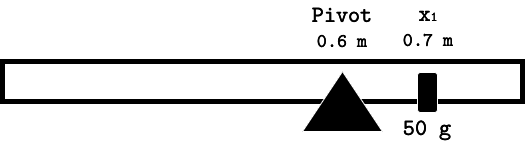
\includegraphics[width=0.75\textwidth]{Scenario3.png}
	\end{center}
\end{figure}

\vspace{-0.5cm}

\begin{table}[H]
\centering
\captionsetup{font=large}
\caption{Scenario 3 - Values}
\label{tab:s3tab}
\resizebox{11cm}{!}{%
\begin{tabular}{@{}cccc@{}}
\toprule
\multicolumn{2}{c}{\textbf{x\textsubscript{com} (m)}}        & 0.6   &  \\ \midrule
\textbf{x\textsubscript{1} (m)}            & \multicolumn{1}{c|}{0.7}    & \textbf{m\textsubscript{1} (kg)} & 0.05 \\
\textbf{x\textsubscript{com} Expected (m)} & \multicolumn{1}{c|}{0.5833} & \textbf{M\textsubscript{T} (kg)} & 0.06 \\ \midrule
\multicolumn{2}{c}{\textbf{x\textsubscript{com} Error (\%)}} & 2.857 &  \\ \bottomrule
\end{tabular}%
}
\end{table}

%----TABLES-----%

%----GRAPHS-----%

%----GRAPHS-----%



